% Шаблон (версия от 15.02.2016) предназначен 
% для использования студентами каф. ПМиИ СамГТУ 
% при оформлении отчетов по лабораторным работам. 
% Для настройки пакета listigs использовался материал 
% статьи Михаила Конника aka virens
% <http://mydebianblog.blogspot.ru/2012/12/latex.html>
% Copyright (c) 2016 by Mikhail Saushkin (msaushkin@gmail.com) 
% All rights reserved except the rights granted by the
% Creative Commons Attribution 4.0 International Licence
% <https://creativecommons.org/licenses/by/4.0/>
% Свежая версия шаблона здесь <https://www.overleaf.com/read/sqvxbnhgxxdm>
\documentclass[14pt,a4paper,report]{ncc}
\usepackage[a4paper, mag=1000, left=2.5cm, right=1cm, top=2cm, bottom=2cm, headsep=0.7cm, footskip=1cm]{geometry}
\usepackage[utf8]{inputenc}
\usepackage[english,russian]{babel}
\usepackage{indentfirst}
\usepackage[dvipsnames]{xcolor}
\usepackage[colorlinks]{hyperref}
\usepackage{listings} 
\usepackage{caption}
\usepackage{amssymb}
\usepackage{tcolorbox}
\DeclareCaptionFont{white}{\color{white}} %% это сделает текст заголовка белым
%% код ниже нарисует серую рамочку вокруг заголовка кода.
\usepackage{color} %% это для отображения цвета в коде
\DeclareCaptionFormat{listing}{\colorbox{gray}{\parbox{\textwidth}{#1#2#3}}}
\captionsetup[lstlisting]{format=listing,labelfont=white,textfont=white}
\lstset{% Собственно настройки вида листинга
inputencoding=utf8, extendedchars=\true, keepspaces = true, % поддержка кириллицы и пробелов в комментариях
language=C++,            % выбор языка для подсветки (здесь это Pascal)
numberstyle =\tiny
basicstyle=\small\sffamily, % размер и начертание шрифта для подсветки кода
keywordstyle =\color{ForestGreen},
numbers=left,               % где поставить нумерацию строк (слева\справа)
numberstyle=\tiny,          % размер шрифта для номеров строк
stepnumber=1,               % размер шага между двумя номерами строк
numbersep=5pt,              % как далеко отстоят номера строк от подсвечиваемого кода
backgroundcolor=\color{white}, % цвет фона подсветки - используем \usepackage{color}
showspaces=false,           % показывать или нет пробелы специальными отступами
showstringspaces=false,     % показывать или нет пробелы в строках
showtabs=false,             % показывать или нет табуляцию в строках
frame=single,               % рисовать рамку вокруг кода
tabsize=2,                  % размер табуляции по умолчанию равен 2 пробелам
captionpos=t,               % позиция заголовка вверху [t] или внизу [b] 
breaklines=true,            % автоматически переносить строки (да\нет)
breakatwhitespace=false,    % переносить строки только если есть пробел
escapeinside={\%*}{*)}      % если нужно добавить комментарии в коде
}

\begin{document}
% Переоформление некоторых стандартных названий
%\renewcommand{\chaptername}{Лабораторная работа}
\def\contentsname{Содержание}

% Оформление титульного листа
\begin{titlepage}
\begin{center}
\textsc{ФГОУ ВО Уральский Федеральный Университет \\ имени первого Президента России Б.Н.Ельцина\\[5mm]
Физико-технологический институт\\[2mm]
Кафедра теоретической физики и прикладной математики}

\vfill

\textbf{ОТЧЁТ ПО ЛАБОРАТОРНОЙ РАБОТЕ №2\\[3mm]
«Моделирование атомной структуры реальных кристаллов»\\[6mm]
}
\end{center}

\hfill
\begin{minipage}{.5\textwidth}
Студент:\\[2mm] 
Вялова С.А.\\
группа: ФтМ-170403 \\[5mm]

Преподаватель:\\[2mm] 
д.ф.-м.н., профессор\\
Мазуренко Владимир Владимирович\\[5mm]

Консультант:\\[2mm] 
н.с.\\
Сотников Олег Михайлович\\

\end{minipage}%
\vfill
\begin{center}
\today  \\
%\theyear\, г.
 Екатеринбург.
\end{center}
\end{titlepage}

% Содержание
\tableofcontents
\newpage
\chapter{Моделирование атомной структуры реальных кристаллов}
\section{Цель работы}


Разработка программы для моделирования основного состояния двумерных решеток, в которых частицы взаимодействуют через потенциал Леннарда-Джонса. Рассмотрение квадратной и треугольной решетки с одинаковой плотностью атомов.
\

В ходе выполнения работы необходимо реализовать следующие пункты:
\begin{itemize}
\item Определить энергии треугольной и квадратной решеток при различных линейных размеров решеток;
\item вычислить плотность системы в каждом случае;
\item выяснить, какова зависимость плотности решетки от линейных размеров решетки;
\item выяснить, энергия какой из рассматриваемых решеток меньше.
\end{itemize}

\

\newpage\section{Теоретическая часть }
\subsection{Потенциал Леннарда-Джонса}
%text
Потенциал Леннарда-Джонса представляет собой простую модель парного взаимодействия неполярных молекул, описывающая зависимость энергии взаимодействия двух частиц от расстояния между ними.
Потенциал был предложен Леннардом-Джонсом первоначально для исследования термодинамических свойств инертных газов. Наиболее часто используется так называемый (6-12)-потенциал Леннарда-Джонса, записанный в форме 
\
\begin{equation}
 U = 4 \cdot \varepsilon \cdot [(\sigma/r)^{12} - (\sigma/r)^{6}  ] ,
 \end{equation} 
где $\varepsilon$ - глубина потенциальной ямы, $\sigma$ - значение расстояния между частицами, при котором потенциал равен нулю. Шестая степень убывания отвечает электростатическому диполь-дипольному и дисперсионному притяжению; двенадцатая степень убывания потенциала моделирует достаточно жесткое отталкивание и выбрана из соображений математического удобства.
\


%\caption{Зависимость температуры системы от шага по времени.}

\newpage
\subsection{Описание  методов}
%text
В ходе работы необходимо исследовать треугольные и квадратные решетки с различными линейными размерами. Пусть $L_x$ - ширина треугольной решетки, $n_c$ - число частиц в каждой строке или столбце. Столбцы треугольной решетки отстоят друг от друга на $a={L_x}/{n_c}$, а каждую строку разделяет расстояние $\frac{\sqrt{3}}{2} a$. В каждой строке узлы смещены на $frac{a}{2}$ относительно предыдущей строки. Высота треугольной решетки составляет $L_y=\frac{\sqrt{3}L_x}{2}$, а общее число частиц в системе составляет $N={n_c}^2$. 
\
Параметры для квадратной решетки подбираются исходя из требования равенства плотностей  треугольной и квадратной решеток. Таким образом, сторона квадратной решетки $L=\sqrt{L_x \cdot L_y}$.
\

Энергия решетки вычисляется через потенциал Леннарда-Джонса следующим образом:
\begin{equation}
E=4 \varepsilon \sum\limits_{i=1}^N \sum\limits_{s=i+1}^N{ [(\sigma/\vec{r}_{is})^{12} - (\sigma/\vec{r}_{is})^{6}  ]}
\end{equation}
\

Плотность решетки вычисляется как частное числа частиц в решетке и полной площади решетки.

Характерный вид расположения атомов в треугольной и квадратной решетках для $L_x=5$ и $L_x=7$ представлен на рисунках \ref{ris:image1} и \ref{ris:image2}. 
\begin{figure}[h]
\center{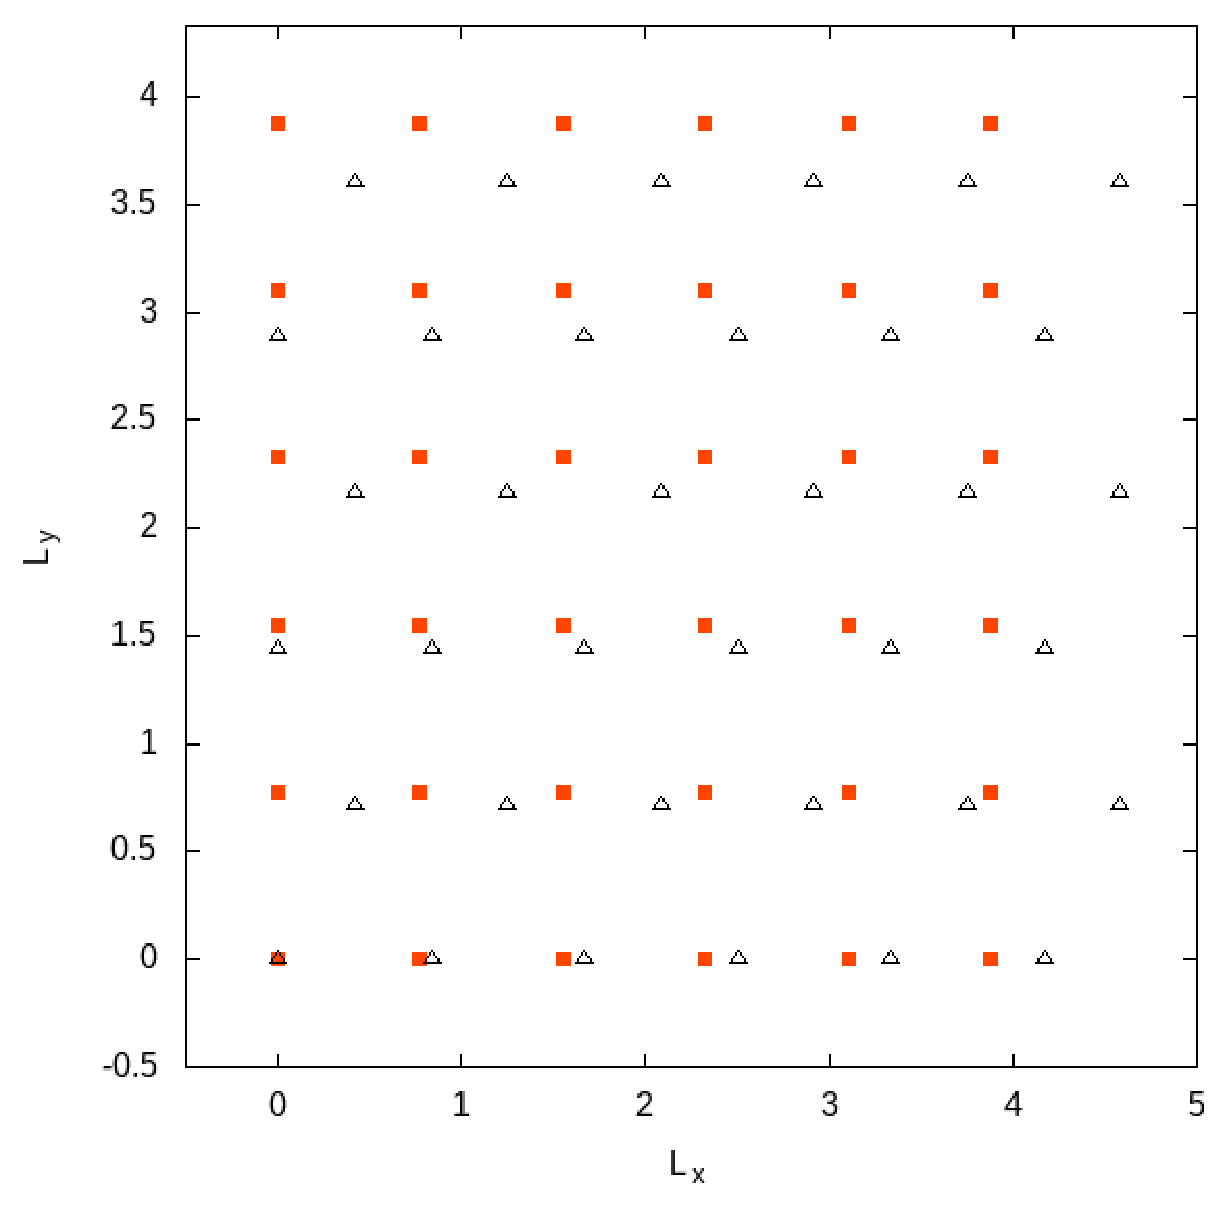
\includegraphics[width=0.6\linewidth]{Lx5}}
\caption{Расположение атомов в треугольной и квадратной решетках для $L_x=5$.}
\label{ris:image1}
\end{figure}
\

\begin{figure}[h]
\center{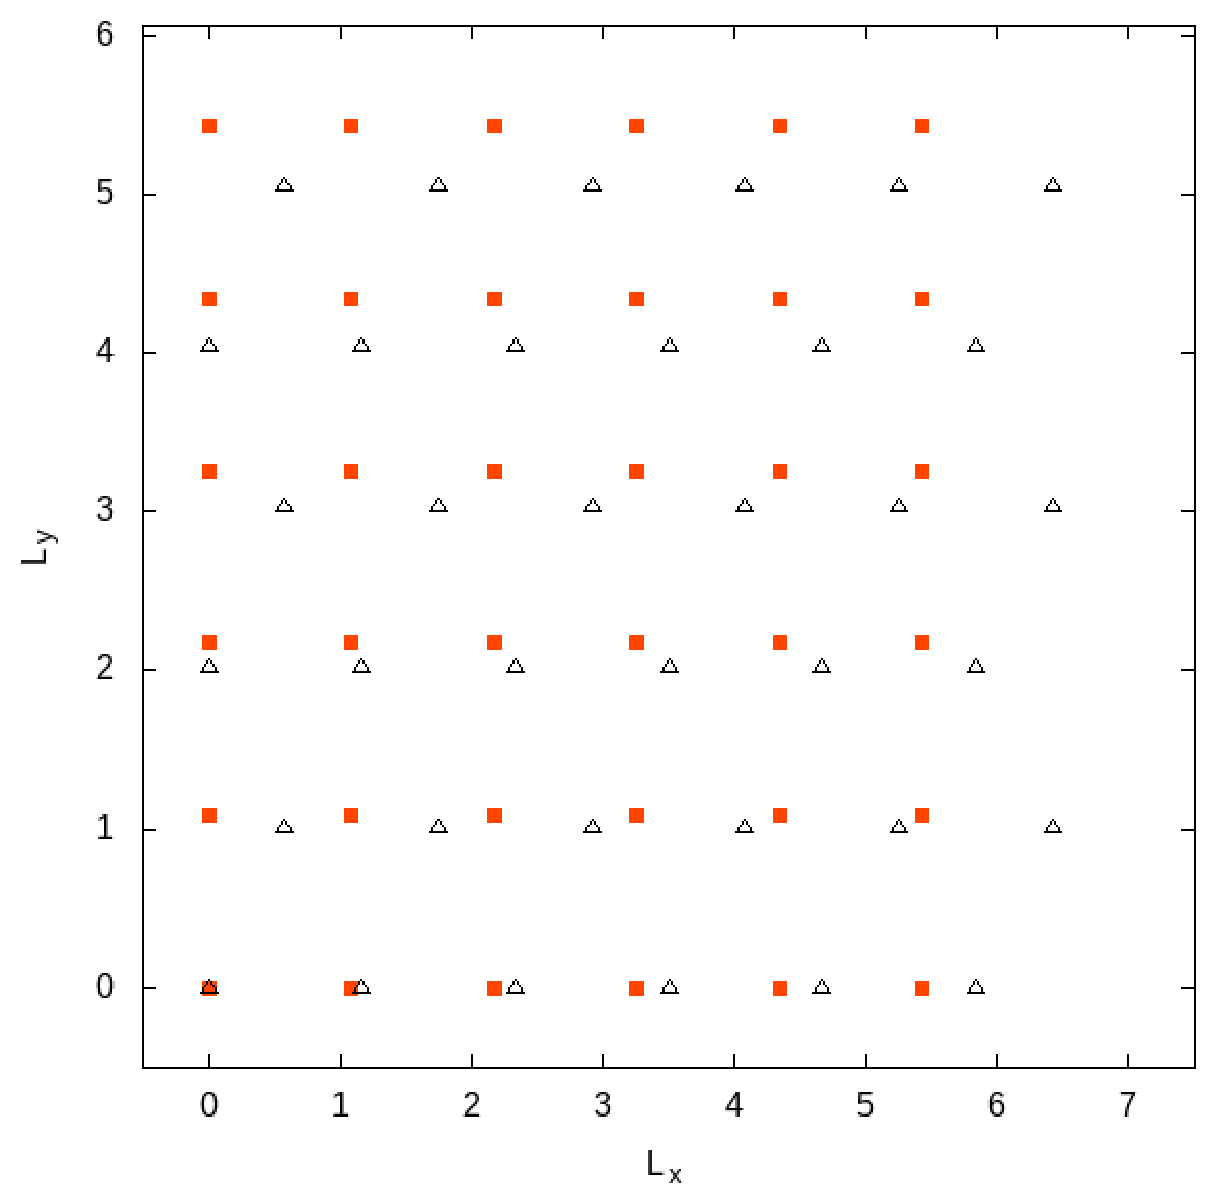
\includegraphics[width=0.6\linewidth]{Lx7}}
\caption{Расположение атомов в треугольной и квадратной решетках для $L_x=7$.}
\label{ris:image2}
\end{figure}
\
\subsection{Разработка программной части}
Для решения поставленной задачи была разработана программа на языке С++. Задача программы - сгенерировать начальные значения координат для треугольной, квадратной решетки с заданными линейными размерами.
Программа последовательно генерирует следующие типы решеток:
\begin{itemize}
\item квадратная, {$L_x=5$}
\item квадратная, {$L_x=7$}
\item треугольная, {$L_x=5$}
\item треугольная, {$L_x=7$}
\end{itemize}
Далее в цикле считается энергия решетки для каждого значения параметра $\sigma$ с шагом $0.001$, вычисляется минимальное значение энергии решетки на интервале $\sigma$ от 0 до 5 и в минимуме фиксируется значение $\sigma$. Значения энергии системы в зависимости от параметра $\sigma$ на каждом шаге моделирования записываются в файл для построения соответствующих графиков зависимости. Для каждой решетки вычисляется плотность. 
Значения минимальной энергии, плотности, значения параметра $\sigma$ в минимуме для каждой решетки выводятся в терминал. 

\ 

При исследовании системы были использованы следующие входные данные:
\begin{itemize}
\item начальное значение параметра $\sigma$: 0;
\item конечное значение параметра $\sigma$: 5;
\item шаг по параметру $\sigma$: 0.001;
\item значение параметра $\varepsilon$=$0.0031$;
\item линейный размер системы по горизонтали ${L_x=5}$;
\item число частиц в строке/столбце ${n_c=6}$;
\item число частиц в решетке ${N={n_c}^2=36}$;
\end{itemize}

Программа запускается из командной оболочки bash. Снимок экрана с выводом программы представлен на рисунке \ref{ris:image3}.
\

\begin{figure}[h]
\center{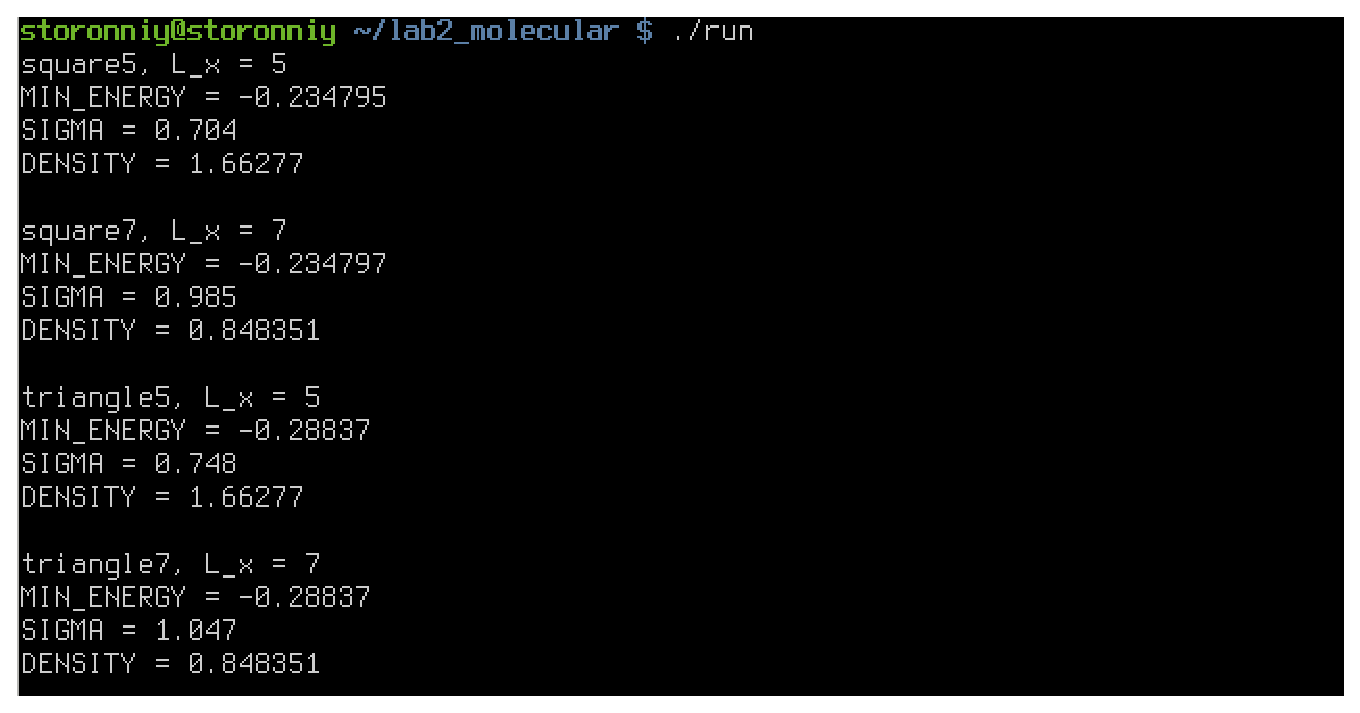
\includegraphics[width=1\linewidth]{program}}
\caption{Демонстрация выполняющейся программы.}
\label{ris:image3}
\end{figure}
\

Как видно из представленного вывода программы, плотности треугольной и квадратной решеток для каждого из исследованных параметров $L_x$, плотности треугольной и квадратной решеток, как и требовалось, равны при одинаковых параметрах $L_x$.
\

Затем необходимо включить динамику для квадратной решетки. 

 \subsection{Результаты моделирования}
В результате моделирования, были получены графики зависимости энергии систем в зависимости от параметра $\sigma$ для каждого значения $L_x$. Соответствующие зависимости представлены на рисунках \ref{ris:image4} и \ref{ris:image5}.


 \
 
 \begin{figure}[h]
\center{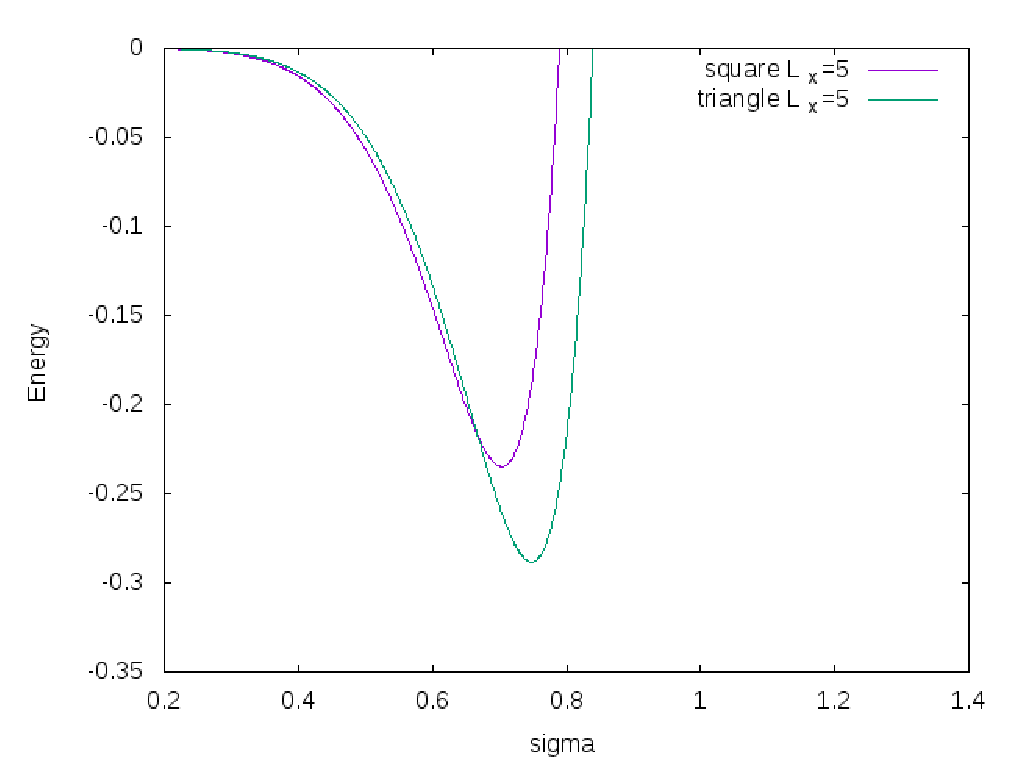
\includegraphics[width=0.6\linewidth]{plot_5}}
\caption{Графики зависимости энергии системы в зависимости от параметра $\sigma$ для треугольной и квадратной решеток для $L_x=5$.}
\label{ris:image4}
\end{figure}
\

  \begin{figure}[h]
\center{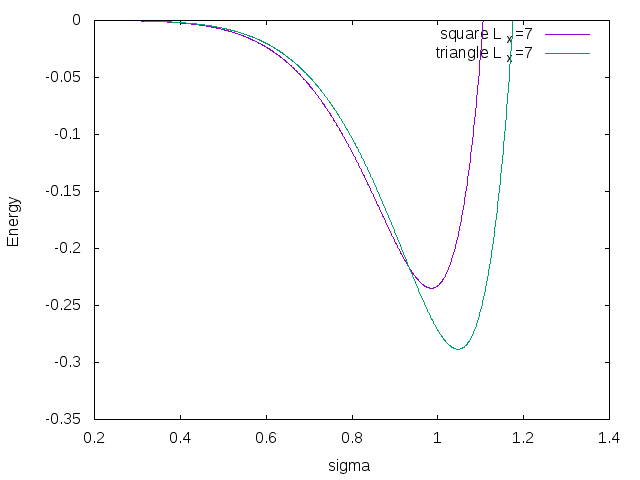
\includegraphics[width=0.6\linewidth]{plot_7}}
\caption{Графики зависимости энергии системы в зависимости от параметра $\sigma$ для треугольной и квадратной решеток для $L_x=7$.}
\label{ris:image5}
\end{figure}
\

После вычисления параметров $\sigma$ в минимуме энергии для каждой решетки необходимо проследить динамику систем частиц для квадратных решеток. Для этого необходимо воспользоваться видоизмененным программным кодом для лабораторной работы №1 (необходимо передать параметры $L_x$ и $L_y$ для периодических граничных условий и на вход подать найденные в ходе данной работы параметры $\sigma$ в минимуме для квадратных решеток), в которой исследвалась динамика двумерной системы частиц, взаимодействующих через потенциал Леннарда-Джонса.
\

Характерный вид состояния системы в начальный момент времени и после некоторого количества шагов динамики системы представлены на рисунках \ref{ris:image6} и \ref{ris:image7}. 
\
\begin{figure}[h]
\center{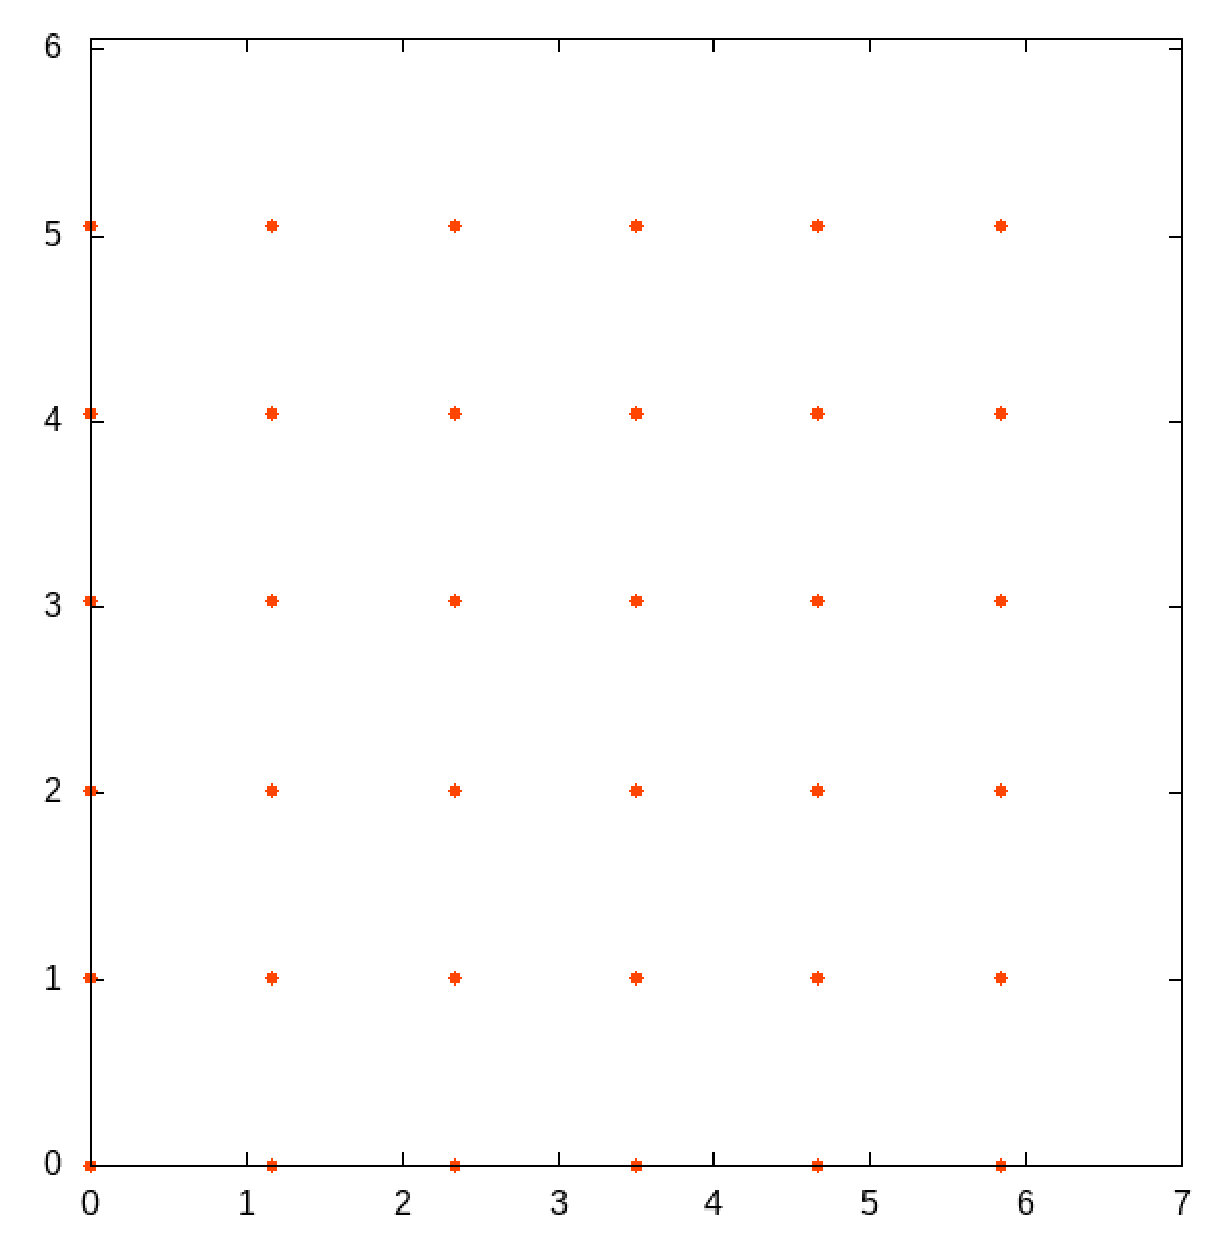
\includegraphics[width=0.6\linewidth]{systemeps}}
\caption{Состояние системы в начальный момент времени для $L_x=7$.}
\label{ris:image6}
\end{figure}
\

\begin{figure}[h]
\center{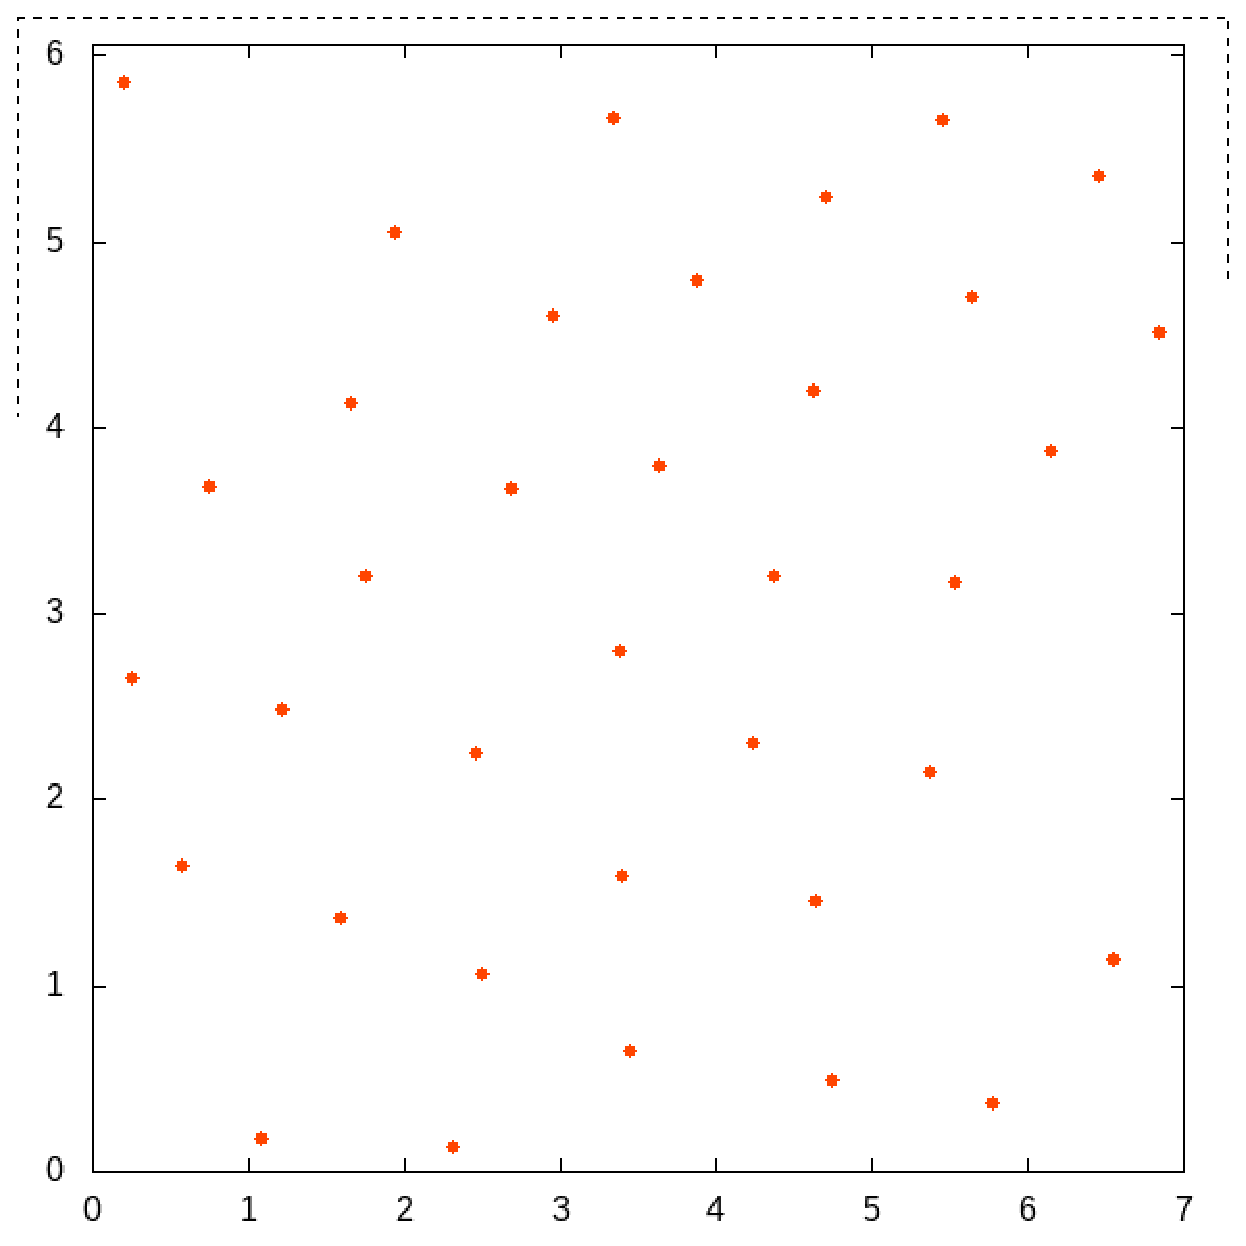
\includegraphics[width=0.6\linewidth]{system_dynamic}}
\caption{Состояние системы после некоторого количества шагов динамики системы для $L_x=7$.}
\label{ris:image7}
\end{figure}
\

Из полученной динамики видно, что после некоторого числа шагов моделирования система приходит к некоторому равновесному состоянию с меньшей энергией, в котором стремится стабилизироваться. Система переходит из квадратного упорядочения к треугольному.
\
Далее былл построен график зависимости энергии системы от числа шагов моделирования, представленный на рисунке \ref{ris:image8}, из которого видно, что полная энергия системы сохраняется, а частицы системы, в попытке привести её в равновесное состояние, испытывают столкновения друг с другом.
\

\begin{figure}[t!]
\center{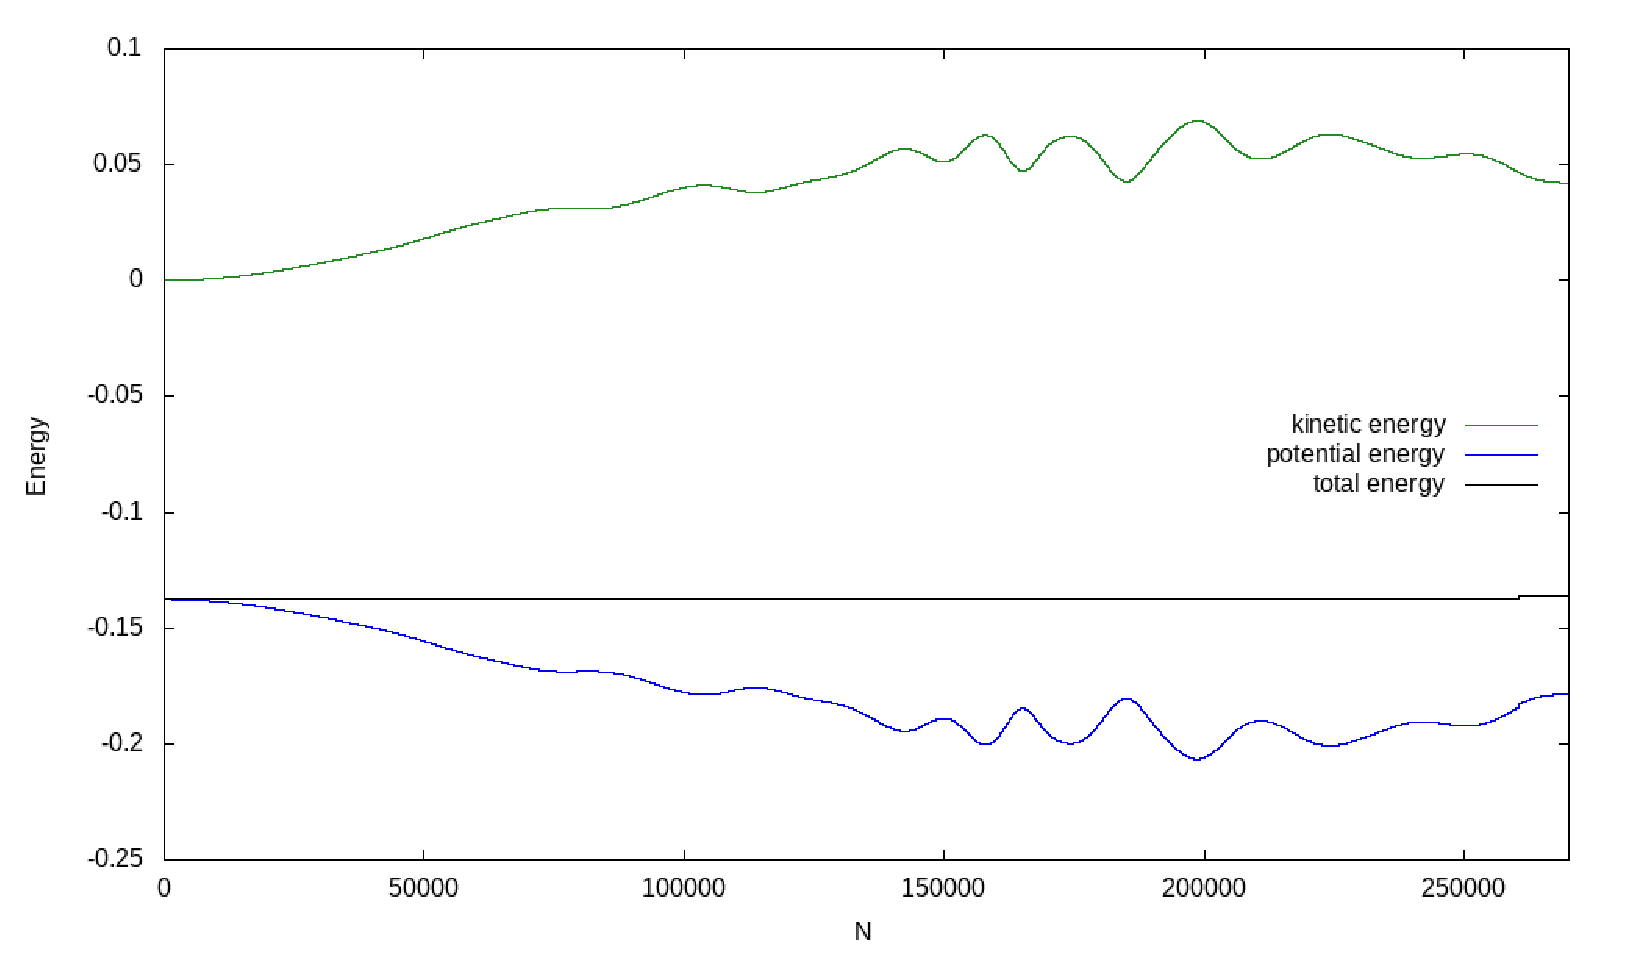
\includegraphics[width=1\linewidth]{system_energy}}
\caption{График зависимости энергии системы от числа шагов моделирования для $L_x=7$.}
\label{ris:image8}
\end{figure}
\


\newpage\section{Выводы}
В ходе данной работы была разработана программа, моделирующая основное состояние треугольной и квадратной решеток, взаимодействующих через потенциал Леннарда-Джонса. Моделирование было проведено для треугольных решеток с линейными размерами системы $L_x=5$ и $L_x=7$, $L_y=\frac{\sqrt{3}}{2} L_x$ и квадратных решеток со стороной $L=\sqrt{L_x \cdot L_y}$, плотности которых равны при одинаковых параметрах $L_x$. 
\
После проведения расчётов были получены изображения,
показывающие расположение частиц в системах, а также были построены и проанализированы графики зависимости энергии систем в зависимости от параметра $\sigma$. Значения $\sigma$, при которых энергия системы с квадратной конфигурацией минимальна, были зафиксированы и квадратные решетки были рассмотрены в динамике с данными значениями $\sigma$. 
\
Из полученных в ходе исследования результатов можно сделать вывод, что треугольная структура решетки является более предпочтительной, поскольку обладает меньшей энергии при том же значении $\sigma$. 
\end{document}
